\vspace*{2em}

\noindent Chapters 3, 4, 5 of the dissertation are comprised of the work carried out in the following papers, respectively:
Please see the flowchart of this thesis on the next page for complete details, 

\begin{enumerate}

\item Testing holography using the lattice with super-Yang-Mills theory on a 2-torus [\href{https://journals.aps.org/prd/abstract/10.1103/PhysRevD.97.086020}{Phys.\ Rev.\ D {\bf 97}, 086020 (2018)}] [\textbf{\textcolor{blue}{\href{https://arxiv.org/abs/1709.07025}{1709.07025}}}]   and,  The properties of $D1$-branes from lattice super Yang--Mills theory using gauge/gravity duality   [\textbf{\textcolor{blue}{\href{https://arxiv.org/abs/1809.00797}{1809.00797}}}] 
 \item Nonperturbative study of dynamical SUSY breaking in $\mathcal{N}$ = (2, 2) Yang-Mills theory  [\href{https://journals.aps.org/prd/abstract/10.1103/PhysRevD.97.054504}{Phys.\ Rev.\ D {\bf 97}, 054504 (2018)}] [\textbf{\textcolor{blue}{\href{https://arxiv.org/abs/1801.00012}{1801.00012}}}]   
   \item On the removal of the trace mode in lattice $\mathcal{N }= 4$ super Yang-Mills theory  [\textbf{\textcolor{blue}{\href{https://arxiv.org/abs/1808.04735}{1808.04735}}}] \href{https://journals.aps.org/prd/accepted/8d072Q69Ide18d24f2c61259a36a4536c02c700b5}{(accepted in Phys Rev. D)}

\end{enumerate}


\vspace{10mm} 


\noindent The following research publications have not been included in the thesis due to their disjoint research field (as of this writing) to the main theme of the dissertation work or 
because of their DOI (Digital object identifier) nature (such as, conference proceedings) :

\begin{enumerate}
\item Tensor renormalization group study of the non-Abelian Higgs model in two dimensions [\textbf{\textcolor{blue}{\href{https://arxiv.org/abs/1901.11443}{1901.11443}}}]  
 \item  Lattice quantum gravity with scalar fields [\textbf{\textcolor{blue}{\href{https://arxiv.org/abs/1810.09946}{1810.09946}}}]
  \item Truncation of lattice $\mathcal{N}$ = 4 super Yang-Mills [\href{https://doi.org/10.1051/epjconf/201817511008}{EPJ Web of Conferences 175, 11008 (2018)}]
   \end{enumerate}


\newpage 

\begin{figure}[tbp]
  \centering
  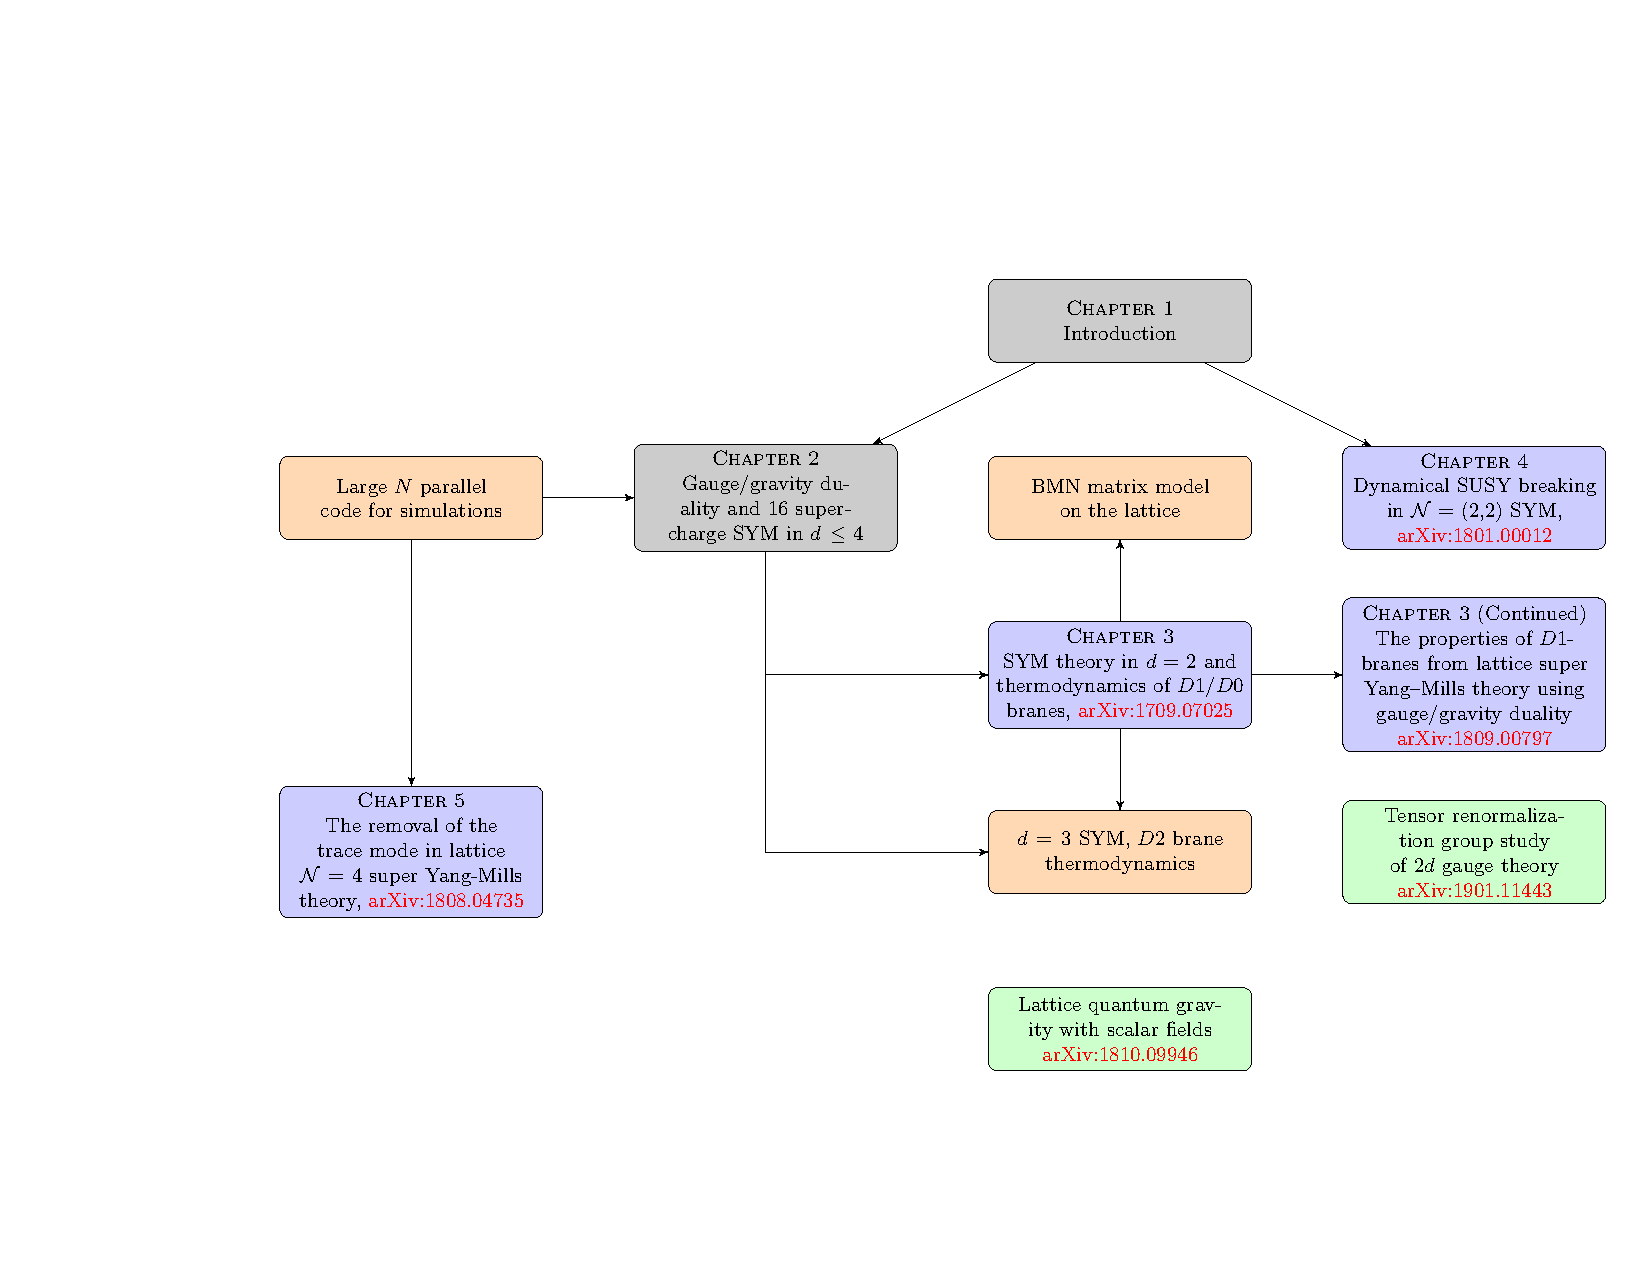
\includegraphics[width=\linewidth]{Figures/Flowchart.pdf}
  \caption{\label{fig:flow1}The grey boxes represent review part of the thesis. The blue boxes are publications that are part of this thesis. The orange boxes represent the work 
  which is in progress and expected to be completed in 2019. The green boxes represent publications (journal article/conference proceedings) that were finished during the Ph.D. but
  are not part of this thesis. }
\end{figure}



